\documentclass[a4paper]{article}

\usepackage[margin=2.5cm]{geometry}
\usepackage{graphicx}

\title{Methods for elimination of crosstalk and inertial effects in bicycle and
motorcycle steer torque estimation}

\author{Jason K. Moore and Mont Hubbard}

\date{September 30, 2013}

\begin{document}

\maketitle

Applying forces to the handlebars of motorcycles and bicycles that result in a
net torque between the front frame and the rear frame (and rider) about the
steer axis provides the most authority of any other input for control of the
lateral dynamics of the vehicles. It has also been postulated that haptic
feedback is very important and may be essential for a human to balance a
bicycle or motorcycle.  Thus is it critical to understand how the steer torque
plays a role in both the open loop and closed loop dynamics of the
bicycle/motorcycle-rider system.

The first portion of the paper will be devoted to a review of steer torque
measurements and modeling results. For example, the earliest measurements of
steer torque were done on a motorcycle \cite{Wilson-Jones1951} with a manual
scale. There have been various sensors designed since to measure steer torque
with various degrees of range and accuracy.

The applied steer torque needed to control a motorcycle is generally much
greater in magnitude than that of a bicycle. For similar maneuvers, motorcycles
may require up to 50 Nm while bicycles require up to 10 Nm. Furthermore, the
rider can easily apply moments to the handlebars up 20 times larger in
magnitude than the steer torque. The sensors must be designed such that these
other forces do not corrupt the much lower magnitude steer torque measurements.

There are several types of designs for measuring steer torque: force
transducers at the hand-handlebar interface, torque transducers on or in the
steer tube, and variations of secondary handlebars connected through
transducers. The merits of each type of design are discussed in the paper.

We show that careful attention must be paid to any steer torque sensors which
measure the strain at points between the hands and the front wheel contact
point.  Depending on the location along the steer axis where the measurement is
made, the inertial effects of the front frame and handlebars between the sensor
and the rider's hands must be accounted for. For bicycles, this is very
important because the torques due to the inertial effects can be a high
percentage of the actual applied torque. No previous steer torque measurements
seem to take this into account.

\begin{figure}
  \centering
  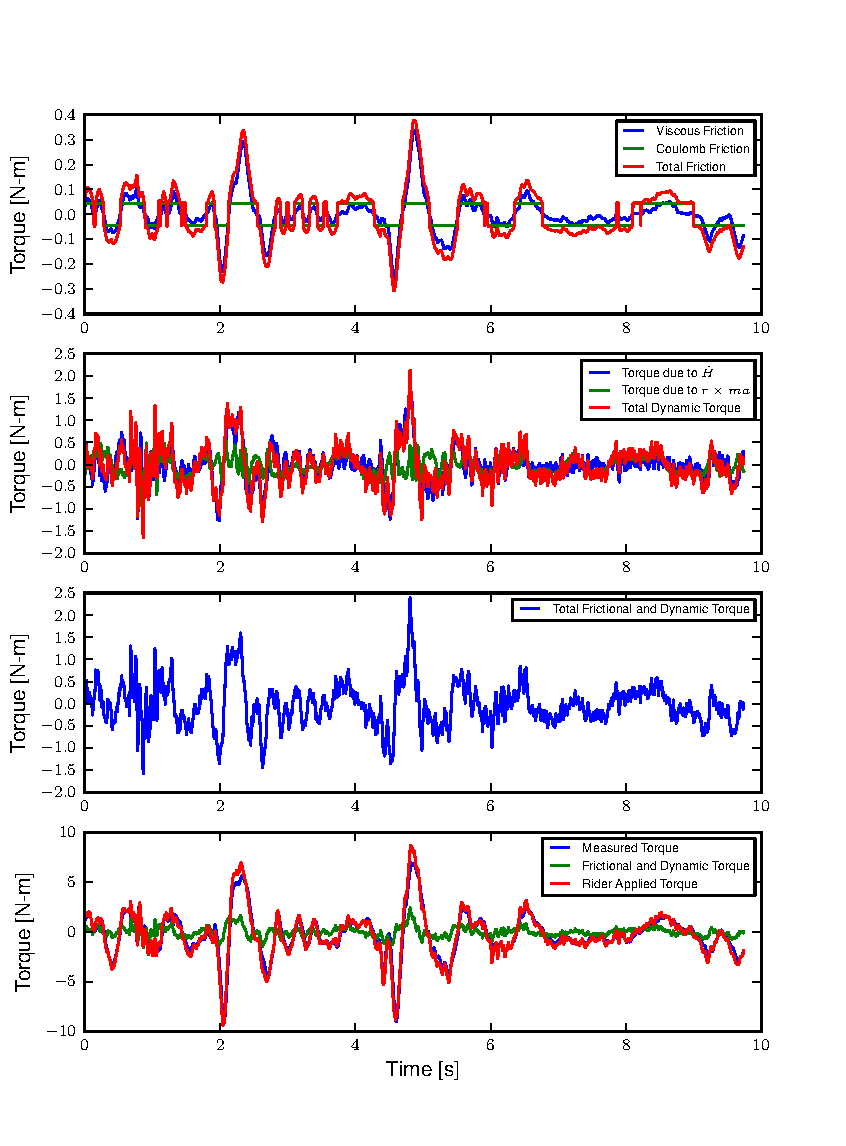
\includegraphics[width=5.0in]{steer-torque-components.pdf}
  \caption{Steer torque components for run \#700. The top plot shows the
  additive viscous and Coulomb friction. The total bearing friction during the
  run is less 0.3 Nm. The second plot shows the torque the rider must apply to
  overcome the handlebar inertia, which is the dominant moment. During peak
  accelerations the additive torque is as high as 1.5 Nm for this run. The
  third plot shows the total additive torque which is as large as 2 Nm. The
  last plot shows the difference in the measured torque and the rider applied
  torque. There are substantial differences, especially at the peaks.}
\end{figure}

Finally, we will describe the steer torque measurement sensor designed for an
instrumented bicycle which attempts to account for many of the flaws of
previous measurements. We include experimental results measuring headset
bearing friction and show results for very accurate torque measurements in
various bicycle maneuvers giving a qualitative and quantitative look at typical
steer torque measurements.

This paper is based on work supported by the National Science Foundation under
Grant No 0928339.

\bibliographystyle{plain}
\bibliography{references}

\end{document}
